
%%%%%%%%%%%%%%%%%%%%%
% A

\appendix
\renewcommand{\thesection}{\arabic{section}}

\chapter{Gannt Diagram}

\begin{figure}[H]
  \centering
    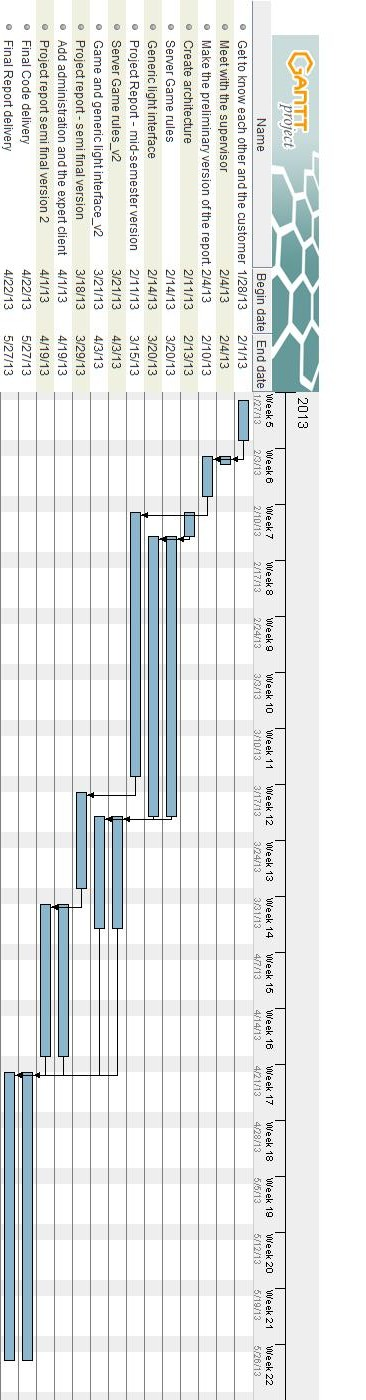
\includegraphics[height=20cm]{img/ganttv3v2.jpg}
  \caption{ 'Gannt diagram'} 
  \label{fig:paperPrototype}
\end{figure}





%%%%%%%%%%%%%%%%%%%%%
% B

\chapter{Don't Panic game rules}
%
\emph{These are the rules of the physical board game, supplied by the customer.}
%
%
\section*{Description of the game}
Don’t Panic is a cooperative game. You start the game as member of a “panic control team”. During your day different potential panicking events will take place and you and your team will have to work together to calm people down and prevent the day from becoming the worst panic event humanity has ever seen. You and your teammates will assume a unique role within the team, with special abilities that will improve your team’s chances, if applied wisely.\\
\\
The aim of the game is to calm the situation down. In the game you can calm people by
\begin{itemize}
	\item opening/blocking paths to help people to get off from frightening situations
	\item talking with them while other solutions are applied
	\item sharing information about how to manage the crisis
	\item moving people from one sector to another. But be careful! You only have a limited time to contain panic.
\end{itemize}
Every 5 minute the “panic level” will increase as a new “panic wave” arrives! If you and your team are unable to keep the panic contained and apply the necessary strategies to calm the people down in time, your city will become a mess and you and your team will lose the game.\\
%
%
\subsection*{A game turn}
The play proceeds clockwise around the table with each player taking turns (in order) until the game ends. For each turn, the current player MUST
\begin{itemize}
	\item take 	4 ACTIONS
	\item draw 	2 INFORMATION CARDS to add to his hand	
	\item draw 	2 EVENT CARDS and perform the corresponding actions on the board
\end{itemize}
%
%
\subsection*{Actions}
A player gets 4 actions to spend on her turn. A given action may be performed more than once during a turn, so long as 1 action is spent for each instance. Each player’s role will grant them special abilities that are unique to that player. Players may also pass if they have nothing else to do. Unused actions CANNOT be saved from turn to turn.\\
\\
In each action the player can
\begin{itemize}
	\item calm 5 people in a sector down
	\item move 5 people from one sector to another
	\item move through a maximum of 3 nodes
	\item create a barrier (is done with the help of another player)	
	\item remove a barrier (is done with the help of another player) 	
	\item decide to spend all his actions in order to create an information center
\end{itemize}
%
%
\subsection*{Components}
1 BOARD represents a real or virtual city. The board is divided into sectors and presents paths and key points. If all the paths in a sector are secured (i.e. blocked) the sector is secured (that is the panic will not augment in the sector at the next wave). However, only a non-secured path can let people pass from one sector to another.\\
\\
8 PAWNS represent the players. The color of the pawn is linked to the draw role card. The pawn moves towards the sectors following key points. The player can act only on the sectors communicating with the key point.\\
\\
1 TIMER calculates the next panic wave. When the timer rings each already panicked sector will be incremented by 5 panicked people (PL). In the non-panicked sectors nothing will happen. During the game panic waves happen initially every 10 minutes, then every 7 minutes and then every 5 minutes.\\
\\
94 PLAYER CARDS :
\begin{itemize}
	\item 6 ROLE CARDS. Each player assumes a specific role in the game which can do particular actions at low cost. The roles are detailed below.
	\item 48 EVENT CARDS. Event cards are, together with the Timer, the source of panic. Each round the player has to draw 2 event cards and apply their effects.
	\item 40 INFORMATION CARDS. Information cards diffuse information which is useful to manage panic. Playing an information card is at 0 cost (i.e. it is an additional action the player can take). Only one card per round can be played and only by the current player. 
\end{itemize}
%
INFORMATION CARDS can be exchanged, but only if the two players are on the same key point. Each round the player has to draw 2 information cards but he can use them only from the next round. Take care! The number of information cards is limited! Once used, they cannot be put back into play.\\
\\
5 INFORMATION CENTERS help lowering the panic. Once an information center has been constructed, the effects of the (draw)?? event cards on the adjacent zone are cut by half. However, creating an information center is a highly costly action. To construct an information center a player needs to use all his actions for this round. A maximum of 5 information centers can be created on a board.\\
\\
DISPLAYS WITH PANIC NUMBERS. Each sector of the game is equipped with a display to indicate the panic level (PL) in the sector. Chain Reactions: Once the panic number reaches quota 50 (that is 50 people panicked in the zone) the panic propagates to all nearby sectors (+5 panicked people). \\
\\
10 BARRIERS help to block the spreading of panic throughout the sectors. To make a zone safe, all the paths have to be blocked. However, people cannot pass through blocked sectors. To create a barrier TWO players have to be on the same key point at the same time. \\
%
%
\subsection*{Sharing Information}
Don’t Panic is a collaborative game! Players are encouraged to openly discuss strategies during the game and share information. An information card can be used only once in a turn but it does not cost any action. Information can be “transferred” from one player to another. To transfer an information card from one player to another, the players have to be on the same key point. Only one card can be transferred at a time. The player who has the role of the Coordinator can transfer a card even if he is not on the same key point. \\
\\
\subsection*{Roles}
Each player is assigned a certain role, and there are six different roles:\\
COORDINATOR : Can share information even if he is not on the same key point\\
CROWD MANAGER: Can calm down 10 people in each sector instead of 5\\
DRIVER: Can move 10 people from one sector to another\\
OPERATION EXPERT: Can create/remove a barrier alone\\
VOLUNTEER: Can support one of the players (apart from the coordinator) duplicating their last action\\
PASSER BY: Can pass 1 information card to a player in an adjacent sector\\
\\
\subsection*{Setting up the game}
\begin{enumerate}
	\item Place the board in the center of the table within easy reach of all the players. Put the displays on the board.
	\item Shuffle the Role cards and deal 1 to each player. Each player takes their corresponding colored pawn. Place the pawn on the big matching colored key point. If the main key point is already taken, choose the small matching colored key point. Put excess Role cards and pawns (if any) back into the box.
	\item Shuffle the INFORMATION CARD cards and deal them to the players face down. For a \\4 PLAYER GAME: 2 CARDS EACH.  \\3 PLAYER GAME: 3 CARDS EACH. \\2 PLAYER GAME: 4 CARDS EACH. \\Place the remaining INFORMATION CARDS face down on the board in the appropriate sector. 	
	\item Shuffle the EVENT CARDS and place them face down on the board in the 	appropriate sector.
	\item Put the initial panic on the board: Each player draws 1 card from the EVENT CARDS and performs the corresponding action.
	\item Turn the INFORMATION CARDS and communicate the possible actions you can perform.
	\item Start the timer.
	\item Play the game! 	
\end{enumerate}

N.B. For a more challenging game session, switch the points 6 and 7. \\
%
\subsection*{Defeat and victory!}
The game ends immediately in defeat for all players if all the map has a panic level higher than 50 panicked people. Players collectively win the game when the panic can no more spread because of the barriers, or if there is no panic on the board.

\section*{User manual}
This is a high level description of how to use the program. When the program starts, the user will have three different choises:

1:	Button - Play

	1.1: A list of active game templates is displayed. Chose one of them, then the program will start a new game with the given template.
	
	1.2: The user can now play the game by moving the players or using actions. 

2: 	Button - Watch replay

	2.1: A list of games that already has been played, is displayed. Chose one of them, then the program will enter the given replay.
	
	2.2: Press the "next" button to show the next action.

3:	Button - Expert interface

	The expert interface is used to set up the game before it is played. 
		
	Button - Add effect, set wanted effect.
	
	Button - Add role, set wanted role.
	
	Button - Add player, set role and startnode for the player.

	Button - Start!, starts the canvas so the user can create the map.

	Mouse click on canvas - adds a new node to the map. 

	Button - Delete node, deletes the selected node from the map.
	
	Button - Start node connection, starts a node connection in the selected zone and connects it to the next node that is selected.
	
	Button - Add zone node, adds a node to a zone. 
	
	Button - Clear zone node, removes a node from a zone. 
	
	Button - Create zone, creates a zone if the nodes around it are zone nodes.
	
	Button - Delete zone, deletes the selected zone.
	
	Button - Set people, sets how many people in the selected zone.
	
 	Button - Set panic, sets the panic level in the selected zone. 






%%%%%%%%%%%%%%%%%%%%%
% C

\chapter{Commentary for meetings with customer}
%
\emph{These are the things discussed and planed at meetings with the customer over the course of the project}
%
%

{\footnotesize
\begin{table}[H]
\begin{tabular}{| p{5cm} | p{10cm} |}\hline
	\textbf{Week}	& \textbf{5} \\ \hline
	Called	By		& Group\\ \hline
	Purpose		& Introduction\\ \hline
	Preparation 
		& Introduction with group first. \\ 
		
	Agenda
		& Lay down the course of the project. \\

	Notes	& -Get familiar with the game, get digital copy of game rules\\ \hline
	
\end{tabular}


\caption{Meeting with customer; 5}
\label{fig:meeting_5}
\end{table}}



{\footnotesize
\begin{table}[H]
\begin{tabular}{| p{5cm} | p{10cm} |}\hline
	\textbf{Date}	& \textbf{7} \\ \hline
	Called	By		& Customer\\ \hline
	Purpose		& Clarify topics within the game, expert, and users.\\ \hline
	Preparation 
		&  Questions are prepared. \\ 
		
	Agenda
		& - Should the expert be able to follow the games progress (in the same room/different room, separate client), or is it enough for the expert to survey the games replay when the game is finished?
	
- Should server be able to communicate with several game sessions (clients) at a time?
	
- Does every player need an account for the game? Login with password?
	
- User profiles? What should they contain? What should the user be able to do himself with his profile? What should be stored?
	
- Disconnect...what should happen to the game session? Should it do a complete stop+delete progress/save state/restart game?
	
- Joining/leaving players. Should a session be able to allow new players in an already running game? Should it allow a player to quit and still continue the game with the other players?
	
- Difference between admin/expert?
		
- Watchers/Expert. Should they be able to remotely view the session? Should he/she be able to write notes in the client when reviewing game replay/watching session?
	
- Should a player be able to write notes while playing the game? Connected to the replay event? Separate document?
		
- Who should have access to replays? Expert, player?.  \\

	Notes	& - 	Expert might decide who should be the different roles before game starts, not just drawing cards in the start of the game!
	SAME ROOM! Should have his own client(laptop) during session for making notes in his interface.
	At least one, perfect solution would be several sessions run on same server.
	Info, statistics, notes expert.
	Save state, then restart at the state later.
	Depending on amount of players (4 or more, can still play). No new players in middle of game.
	Admin=Technical, IT guy. Nothing do with game.
	Redundant, see above. Player should be able to write notes while watching replays.
	Write/store in log in profile after the game.
	Public for users, his own games. Can share replay with others (expert can share?).\\ \hline
	
\end{tabular}

\caption{Meeting with customer; 7}
\label{fig:meeting_7}
\end{table}}


{\footnotesize
\begin{table}[H]
\begin{tabular}{| p{5cm} | p{10cm} |}\hline
	\textbf{Week}	& \textbf{8} \\ \hline
	Called	By		& Customer\\ \hline
	Purpose		& Requirements\\ \hline
	Preparation 
		& Questions regarding requirements. \\ 
		
	Agenda
		& Clarify what the game should do, how to implement, requirements for database. \\

	Notes	& - The game should be as close to to original ass possible, also wants to implements users and game masters. Database should be hosted.\\ \hline
	
\end{tabular}


\caption{Meeting with customer; 8}
\label{fig:meeting_8}
\end{table}}


{\footnotesize
\begin{table}[H]
\begin{tabular}{| p{5cm} | p{10cm} |}\hline
	\textbf{Week}	& \textbf{10} \\ \hline
	Called	By		& Customer\\ \hline
	Purpose		& Ask questions regarding the game rules, show prototype of game\\ \hline
	Preparation 
		& Finish the prototype so it looks OK. Prepare questions for customer regarding rules of the game \\ 
		
	Agenda
		& Customer notifyes us abut timer and cards, that we should implement this for next meeting. Otherwise happy about our progress  \\

	Notes	& - Keep working on the game, focusing on implementing timer and card functionality\\ \hline
	
\end{tabular}


\caption{Meeting with customer; 10}
\label{fig:meeting_10}
\end{table}}


{\footnotesize
\begin{table}[H]
\begin{tabular}{| p{5cm} | p{10cm} |}\hline
	\textbf{Week}	& \textbf{11} \\ \hline
	Called	By		& Customer\\ \hline
	Purpose		& Update on where we are with the project.\\ \hline
	Preparation 
		& Implemented timer and cards (at least core functionality of cards), a task given to us on prior meeting. \\ 
		
	Agenda
		& Discussed how the amount of people should affect the panic level in the zones. Panic in a zone COULD be proportional to amount of people, not important. Discussed events and how they could be solved by finishing a "quest" of different steps (example: if there is a fire: move people out, block zone, put out fire). These "quests" were not a requirement, just a suggestion. Discussed use of Sifteo Cubes (an interactive game system with electronic gadgets) as a client. This was only an experiment, and not a requirement. It is important that we have a working game+client; other clients are "bonuses".  \\

	Notes	& - This week we will work with the report, not the game. This was explained to the customer\\ \hline
	
\end{tabular}


\caption{Meeting with customer; 11}
\label{fig:meeting_11}
\end{table}}



{\footnotesize
\begin{table}[H]
\begin{tabular}{| p{5cm} | p{10cm} |}\hline
	\textbf{Week}	& \textbf{12} \\ \hline
	Called	By		& Customer\\ \hline
	Purpose		& Progress\\ \hline
	Preparation 
		& Create a working version of the newest implementations \\ 
		
	Agenda
		& Clarify the new implementations, get feedback. \\

	Notes	& - Feedbacks are good, customer is satisfied.\\ \hline
	
\end{tabular}


\caption{Meeting with customer; 13}
\label{fig:meeting_12}
\end{table}}


{\footnotesize
\begin{table}[H]
\begin{tabular}{| p{5cm} | p{10cm} |}\hline
	\textbf{Week}	& \textbf{14} \\ \hline
	Called	By		& Customer\\ \hline
	Purpose		& Progress\\ \hline
	Preparation 
		& Prepare questions for customer. \\ 
		
	Agenda
		& Show the newest progress, plan next weeks implementation. \\

	Notes	& - Feedbacks are good. Customer wants us to start on a additional mini project sifteo cubes, we will try to implement it to the code..\\ \hline
	
\end{tabular}


\caption{Meeting with customer; 14}
\label{fig:meeting_14}
\end{table}}


{\footnotesize
\begin{table}[H]
\begin{tabular}{| p{5cm} | p{10cm} |}\hline
	\textbf{Week}	& \textbf{15} \\ \hline
	Called	By		& Customer\\ \hline
	Purpose		& Progress\\ \hline
	Preparation 
		& Prepare questions for customer. Get a working version of the code.\\ 
		
	Agenda
		& Show the newest progress, get feedback from the customer on the new features. \\

	Notes	& - Feedbacks are good, but we should start work on the sifteo cubes as soon as possible.\\ \hline
	
\end{tabular}


\caption{Meeting with customer; 15}
\label{fig:meeting_15}
\end{table}}


{\footnotesize
\begin{table}[H]
\begin{tabular}{| p{5cm} | p{10cm} |}\hline
	\textbf{Week}	& \textbf{17} \\ \hline
	Called	By		& Customer\\ \hline
	Purpose		& Progress\\ \hline
	Preparation 
		& Prepare questions for customer. Show the newest version the expert interface.\\ 
		
	Agenda
		& Show the newest progress, get feedback from the customer on the new expert interface. \\

	Notes	& - Feedbacks are good, but the expert interface should be more intuitive. The customer wants sound effects added to the game, especially mentioned are the sound effects for the timer. Meeting for the sifteo cubes id planned.\\ \hline
	
\end{tabular}


\caption{Meeting with customer; 17}
\label{fig:meeting_17}
\end{table}}


{\footnotesize
\begin{table}[H]
\begin{tabular}{| p{5cm} | p{10cm} |}\hline
	\textbf{Week}	& \textbf{18} \\ \hline
	Called	By		& Customer\\ \hline
	Purpose		& Progress\\ \hline
	Preparation 
		& Prepare a working version of the game, for the customer to try her self. We will have the customer go through the system usability tests.\\ 
		
	Agenda
		& Show the newest progress, new version of expert interface, new sound effects, and sound track, new colors, new game master feature. Have the customer play the game. \\

	Notes	& - Feedback from the newest implementations are great. The customer is very happy with the new sound effects. Some improvements are needed for the expert interface. We explain that there will be no new implementation for the game, but only modifying and making the game more sable.\\ \hline
	
\end{tabular}


\caption{Meeting with customer; 18}
\label{fig:meeting_18}
\end{table}}


%%%%%%%%%%%%%%%%%%%%%
% D

\chapter{Commentary for meeting with supervisor}
%
\emph{These are the commentary for the meetings with our supervisor}
%
%



{\footnotesize
\begin{table}[H]
\begin{tabular}{| p{5cm} | p{10cm} |}\hline
	\textbf{Week}	& \textbf{6} \\ \hline
	Called	By		& Group\\ \hline
	Purpose		& First meeting\\ \hline
	Preparation 
		& Meeting with customer. Thoughts on technology and tools.\\ 
		
	Agenda
		& Discuss initial strategy, process model, tools and frameworks. \\

	Notes	& - See if there exits usable framework for our game. \\ \hline
	
\end{tabular}


\caption{Meeting with supervisor; 6}
\label{fig:s_meeting_6}
\end{table}}

{\footnotesize
\begin{table}[H]
\begin{tabular}{| p{5cm} | p{10cm} |}\hline
	\textbf{Week}	& \textbf{8} \\ \hline
	Called	By		& Group\\ \hline
	Purpose		& Second meeting, feedback form supervisor.\\ \hline
	Preparation 
		& Delivered preliminary report.\\ 
		
	Agenda
		& Discuss strategy, feedback for preliminary report and activity log, the progress. \\

	Notes	& - Cover page, title liste of group mambers missing.\\
& - highlevel chapters mergin, project management.\\
& - justify the text (adjust the text/make it "look nice"?).\\
& - reqirement (functional/non-functional) need improvement, more structures, more use cases, common misunderstading.\\
& - non fun req, importance, What is important? Security, user friendlyness, explain.\\
& - look for ieee stantands for non funq req, guidence.\\
& - decided milestones, for whole semester.\\
& - risk list's remove, network failure, risk list need more work.\\
& - activity template, really important, not in main report, every week \\ \hline
	
\end{tabular}


\caption{Meeting with supervisor; 8}
\label{fig:s_meeting_8}
\end{table}}


{\footnotesize
\begin{table}[H]
\begin{tabular}{| p{5cm} | p{10cm} |}\hline
	\textbf{Week}	& \textbf{12} \\ \hline
	Called	By		& Group\\ \hline
	Purpose		& Feedback for midterm report.\\ \hline
	Preparation 
		& - none\\ 
		
	Agenda
		& Feedback for midterm report. \\

	Notes	& - Project management 2nd chapter.\\
& - Design and architecture instead of implementation\\
& - Requirements after prestudy\\
& - Adjust the text\\
& - More concrete funct. requirements, all features of the software, table of funct. req, id and link.\\
& - Server should not be user (usecase).\\
& - More detailed use cases.\\
& - 2.2 iso usability or operability? portability or transportability.\\
& - Requirements wbs.\\
& - Lessons learned, at the end.\\
& - Reflect the roles and task assignment.\\
& - Two different views on client server architecture. Pattern server/client pga non fun. req.\\
& - Add test result \\ \hline
	
\end{tabular}


\caption{Meeting with supervisor; 12}
\label{fig:s_meeting_12}
\end{table}}


{\footnotesize
\begin{table}[H]
\begin{tabular}{| p{5cm} | p{10cm} |}\hline
	\textbf{Week}	& \textbf{15} \\ \hline
	Called	By		& Group\\ \hline
	Purpose		& Progress and supervision\\ \hline
	Preparation 
		& - none\\ 
		
	Agenda
		& Show supervisor our progress, with report and game development. \\

	Notes	& - Report is to be handed in 19.04.2013, for a semifinal feedback. Talked about the progress of the group, and difficulties. \\
	& - Update lessons learned.\\ \hline
	
\end{tabular}


\caption{Meeting with supervisor; 15}
\label{fig:s_meeting_15}
\end{table}}


{\footnotesize
\begin{table}[H]
\begin{tabular}{| p{5cm} | p{10cm} |}\hline
	\textbf{Week}	& \textbf{17} \\ \hline
	Called	By		& Group\\ \hline
	Purpose		& Feedback for semi final report.\\ \hline
	Preparation 
		& - none\\ 
		
	Agenda
		& Feedback for semi final report. \\

	Notes	& - New Chapter: "Iteration", after design an architecture. Show progress through iterations.\\
& - Put all status reports in the appendix, in addition to having example in chapter 2.\\
& - Link ALL use cases to the Functional requirements.\\
& - Add test results, preferably with customer participating and accepting.\\
& - Link ALL tests and test results to functional requirements.\\
& - Write chapter 7 and 8, most important chapters.\\ \hline
	
\end{tabular}


\caption{Meeting with supervisor; 17}
\label{fig:s_meeting_17}
\end{table}}